\section{Results and Discussion}
\label{sec:discussion}

This section presents and discusses the results of the simulations, structuring the analysis on multiple levels to provide an overview of the behavior of LLM agents within the simulated environment.

The analysis starts with the distribution of coalitions in the populations, as it may influence the following observations, and proceeds with some examples of the final network structures that emerged.
Then, the focus shifts to the analysis of interactions, exploring how agents behave toward different groups and whether there are differences between base users and misinformation agents.
This is followed by an analysis of the opinion evolution, including an exploration of the potential impact of misinformation on opinion shifts.
A toxicity analysis is then conducted to assess the tone of the conversations generated in the simulations.
Finally, some overall considerations regarding the effects of the different the content recommender systems are provided.


% Population composition
\subsection{Coalition Distribution in the Population}
At the beginning of the simulation, users are initialized with data from real-world users, including their political leaning, by randomly sampling from the dataset.
This approach allows the simulated population to reflect the distribution of the coalitions observed in the real data.

As shown in Figure \ref{fig:population}, the distribution of coalitions is not balanced.
Specifically, the Right coalition has the largest number of users, followed by Centre-Left and Third Pole, which have similar sizes.
In contrast, the M5S group is smaller, with low variability across different simulations.

It's important take into consideration this imbalance in the following analyses, as it may influence both the absolute volume of interactions and some of the emerging dynamics in the system.


\begin{figure}[h]
    \centering
    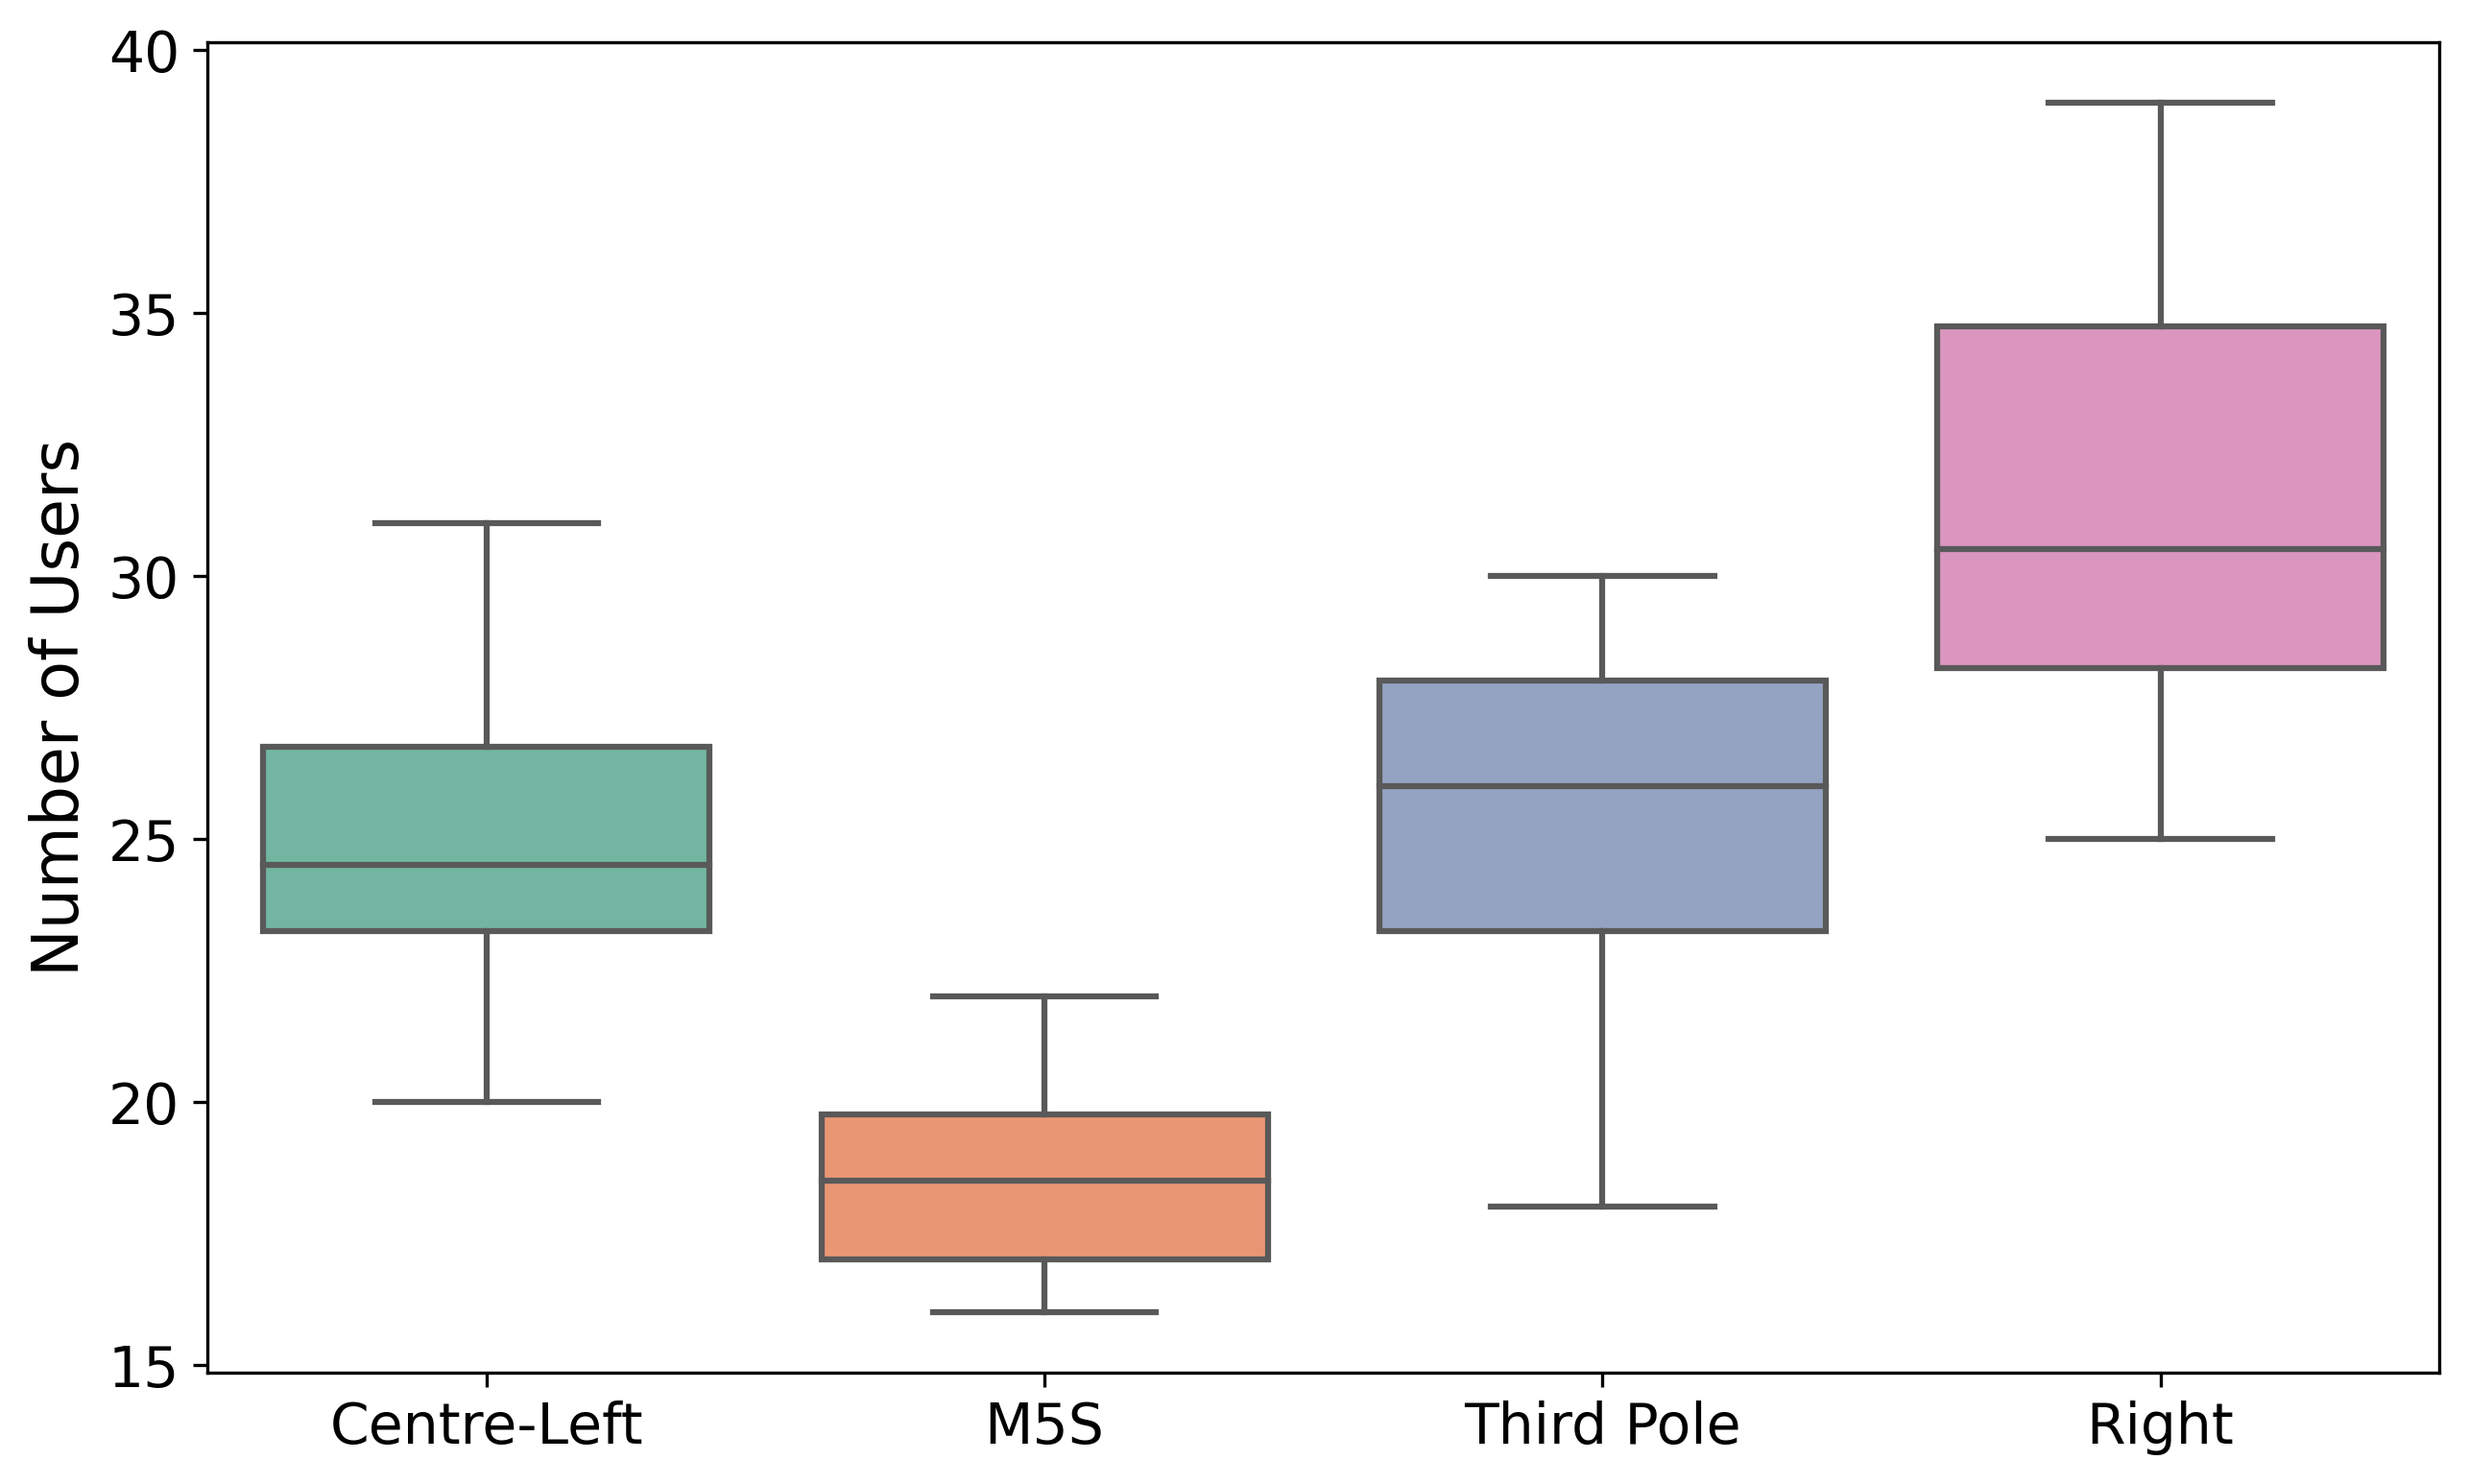
\includegraphics[width=0.6\linewidth]{Images/Network/population_composition_DefaultRecSys.png}
    \caption{Distribution of the number of agents per political coalition in the simulations.
    The Right coalition has the largest number of users, followed by Centre-Left and Third Pole.
    The M5S coalition has the smallest number of agents, with low variability across simulations.}
    \label{fig:population}
\end{figure}


% Network
\subsection{Network structure}
At the beginning of the simulation, users are not connected: the social network starts in an empty state.
The network structure emerges over time, based on the interactions of the individuals: each time an agent interacts with another user, for instance by reading a post, it can decide to follow the author.
This mechanism replicates a realistic dynamic of the evolution of the network, which evolves according to the preferences and behavior of the agents.

\medskip
In Figure \ref{fig:network_structure} there are four examples of final networks generated by simulations with the default recommender system, but with different levels of misinformation.

Nodes are colored according to the supported coalition, while the bold borders indicate misinformation agents.
The network is not split into isolated groups: agents connect not only with members of the same coalition, but also with users from opposing coalitions, including misinformation agents.
This suggests that, at a structural level, the interaction among different groups are present even with users producing misleading content.

Moreover, some nodes look bigger, due to the higher number of connections they have.
This is valid also for some misinformation agents, confirming that they can have a realistic behavior and become central in the network.

\begin{figure}[h]
    \centering
    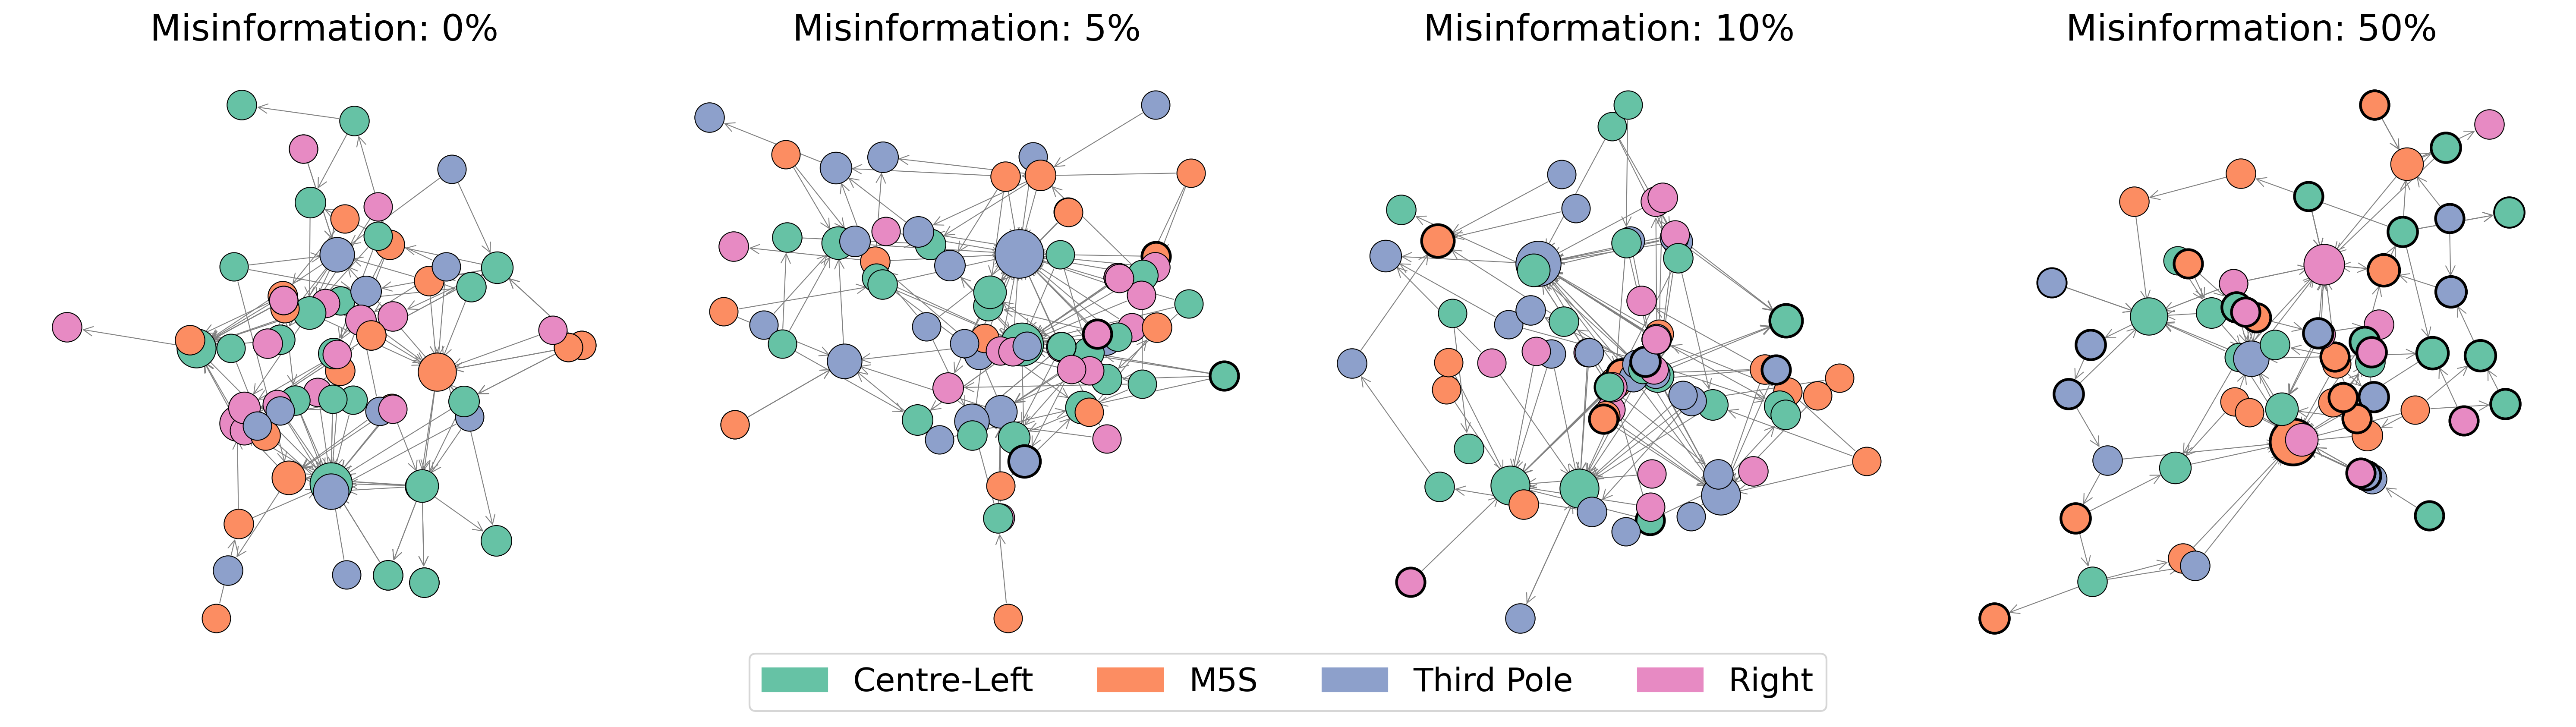
\includegraphics[width=1\linewidth]{Images/Network/graphs_DefaultRecSys.png}
    \caption{Final structure of the social network in four simulations with different levels of misinformation. 
    Nodes are agents, colored according to the supported coalition; the bold borders indicate misinformation agents. 
    The dimension of the nodes indicates the number of connections of an agent.
    The connections in the network are both in and out coalition, including misinformation agents.}
    \label{fig:network_structure}
\end{figure}


% Interactions
\subsection{Interactions}
An interesting aspect to analyze is how users interact during the simulations.
The possible interaction types are: \textit{post}, \textit{comment}, \textit{like}, \textit{dislike}, \textit{follow}, and \textit{unfollow}.
The analysis is divided into two parts.
First, a comparison between in-group and out-group interactions across coalitions is performed, in order to see whether users behave differently depending on the political group they interact with.
Then, the activity for each interaction type is analyzed, comparing base users and misinformation agents, to investigate whether the two groups have different behaviors.

\subsubsection{In-group and out-group interactions across coalitions}
To analyze how users interact with supporters of the same coalition compared to those from other groups, four types of interactions have been considered: \textit{like} and \textit{follow} (positive interactions), \textit{dislike} and \textit{unfollow} (negative interactions).

Figure \ref{fig:interactions_inout} shows, for each coalition, the percentage of interactions directed toward the in-group (users of the same coalition) compared to out-groups, distinguishing between positive and negative interactions.

Looking at the positive interactions, the Centre-Left and Third Pole coalitions show a balanced behavior, with around half of their likes and follows directed toward users of their own group.
In contrast, M5S and Right show fewer in-group positive interactions.
For M5S, this may be explained by the smaller size of the group in the simulated populations, as already discussed in Figure \ref{fig:population}, which increases the likelihood of interacting with out-group users.
However, this doesn't apply to the Right, which includes a larger number of agents. In this case, users seems to be more inclined to like and follow users of other coalitions.

For what concerns the negative interactions, these are mostly directed toward users of other coalitions.
In-group negative interactions are low for all coalitions, with the exception of the Right, which shows higher values with respect to other groups.

By comparing in-group positive and negative interactions, it's possible to observe that most coalitions tend to prefer positive interactions with members of the same group.
The only exception is the Right, where the in-group negative interactions are more frequent than the positive ones.
This might indicate a greater level of internal fragmentation: even among users with similar political views, conflicts or disagreements seem to emerge more often.


\begin{figure}[h]
    \centering
    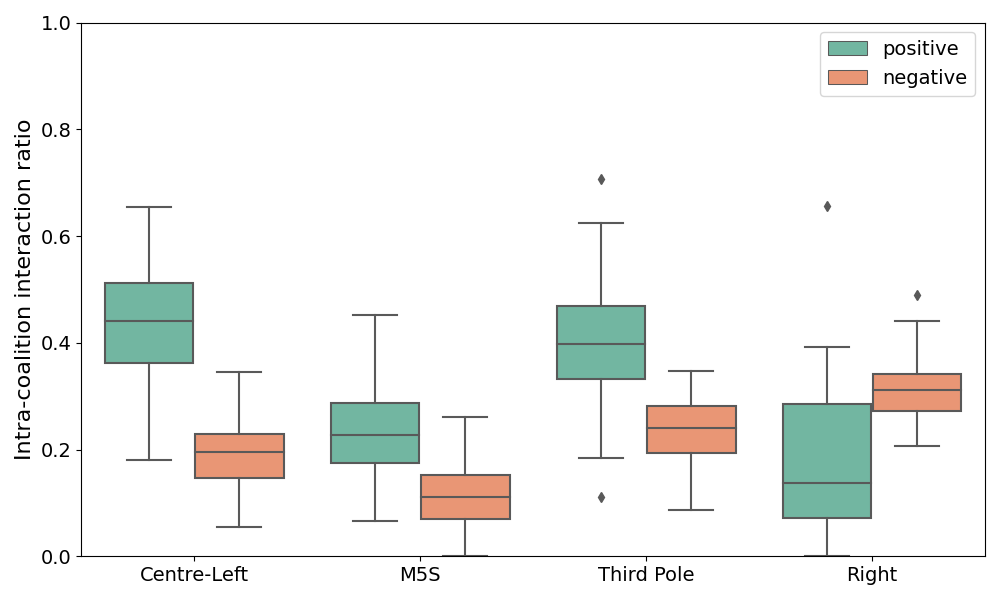
\includegraphics[width=0.6\linewidth]{Images/Interactions/pos_neg_in_DefaultRecSys.png}
    \caption{Percentage of interactions directed toward the same group (in-group), divided into positive interactions (\textit{like}, \textit{follow)}) and negative interactions (\textit{dislike}, \textit{unfollow}), for each coalition.
    Centre-Left and Third Pole show balanced in and out interactions, while M5S and Right have higher positive out-group interactions.
    The Right Coalition is the only one where the in-group negative interactions are more than the positive ones, indicating a possible internal fragmentation.}
    \label{fig:interactions_inout}
\end{figure}


\subsubsection{Interaction activity per user type}
Figure \ref{fig:interactions_count} shows the number of interactions per user, comparing base and misinformation agents.
By looking at the interactions related to content generation, it's possible to notice that \textit{posts} are more frequent among misinformation agents.
The same is true for \textit{comments}, which represents the most used interaction for both groups.

As for \textit{like} reactions, there are not evident differences: the distribution for the two groups overlap, indicating a similar behavior in showing appreciation to read content.

\textit{Dislikes} are instead the most frequent interaction among the ones with don't include content creation.
Base users generally perform more dislikes compared to the other group, suggesting that they tend to express disagreement more frequently.

Looking at the network dynamics, \textit{follows} are significantly lower for misinformation agents, which often don't create any connection during the simulation, while base users then to form more connections.
\textit{Unfollow} actions are instead almost absent for both groups. This is likely because the network starts without preexisting connections, and the simulated time allows the network to emerge but not to evolve significantly in terms of link removal.

Another interesting aspect is the presence of several outliers, especially for comments, posts and dislikes, indicating some users are particularly active.

Overall, these results highlight that misinformation agents are highly active in content generation but are less engaged in building social connections.


\begin{figure}[h]
    \centering
    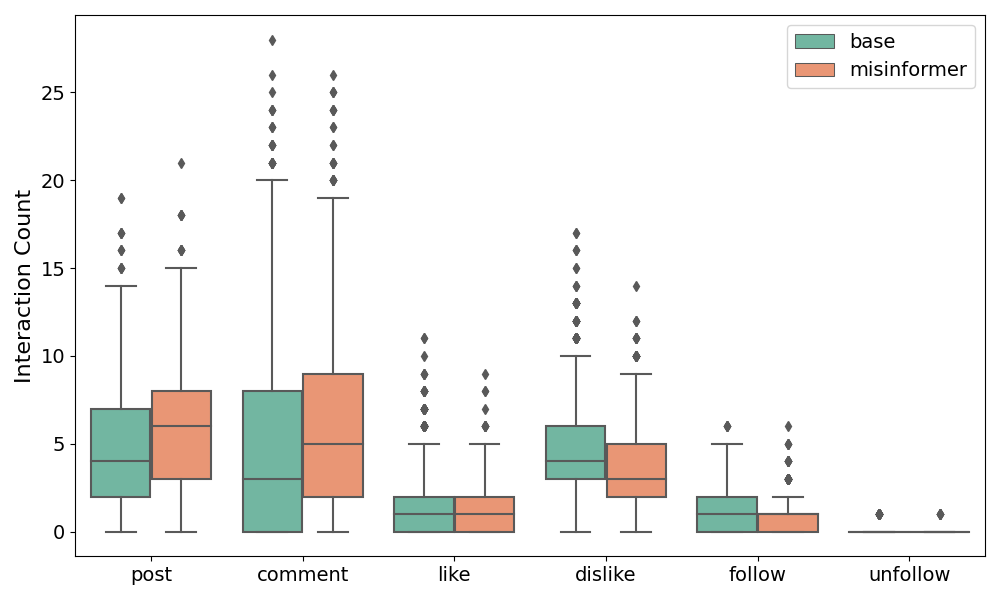
\includegraphics[width=0.6\linewidth]{Images/Interactions/count_per_user_DefaultRecSys.png}
    \caption{Number of interactions per user, distinguishing by base and misinformation agents.
    Among the six interaction types shown, \textit{comments} are the most frequent, followed by \textit{posts} and \textit{dislikes}.
    Base agents tend to perform more dislikes and follows compared to misinformers, whereas the number of \textit{unfollows} is negligible for both groups.
    Misinformation agents are more active with posts and comments, but build less connections.
    Outliers indicate the presence of very active users.
    }
    \label{fig:interactions_count}
\end{figure}


% Opinion
\subsection{Opinion evolution}
One of the main aspects of the simulations is the evolution of opinions over time, which can be observed making a distinction for each topic and coalition.
Figure \ref{fig:opinion_evolution} shows the opinion evolution over virtual days, with a 95\% confidence interval, on each setup.
The plots on the top represent the score directly assigned by LLMs, while the ones on the bottom show the score computed with traditional opinion dynamic models.

Comparing the two score models highlights a high coherency in the trends: both scores evolves with the same behavior, and with similar mean values.
This suggests that LLMs are able to effectively replicate the opinions updates at the population level, as the observed behavior is close to that of established models in literature. Therefore, LLMs represent a valid approach in complex scenarios.

Across all topics, it's possible to observe a progressive convergence of opinions toward neutral values, indicating that agents trend to reduce their polarization over time.
It would be interesting to extend the duration of the simulations, as it would allow to determine if this trend persists or stabilizes.

Moreover, the general trend is the same even in different setups (with varying misinformation levels and different recommender systems), confirming the validity of these observations.

\begin{figure}[h]
    \centering
    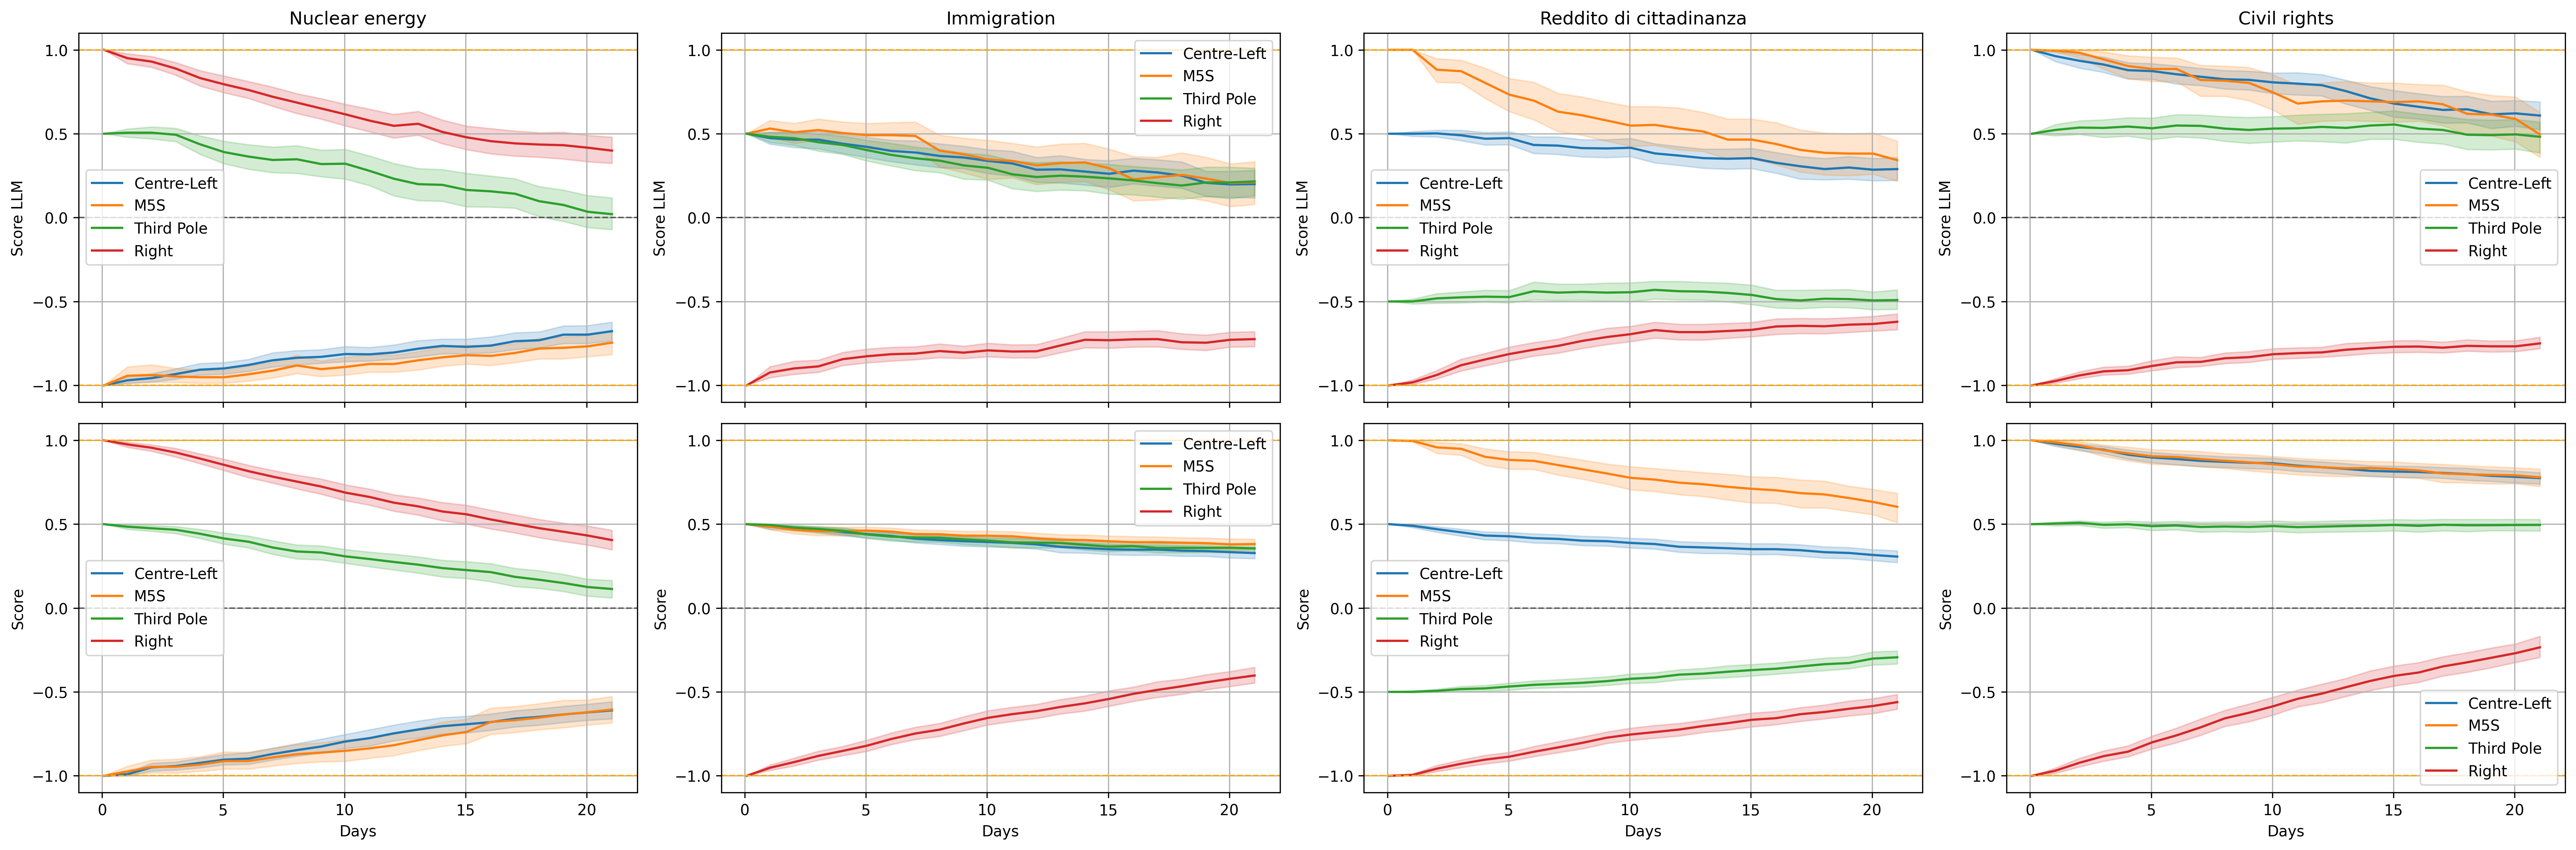
\includegraphics[width=1\linewidth]{Images/Opinions/d21a100m00d_DefaultRecSys.png}
    \caption{Evolution of opinion for each topic, comparing LLM-assigned score (\textit{score\_llm}, top row) and the one assigned by a traditional model (\textit{score}, bottom row).
    Each line represents a coalition, with a 95\% confidence interval.
    This figure is based on the runs for a single setup, but the trend is consistent with the other scenarios.}
    \label{fig:opinion_evolution}
\end{figure}


% Misinformation
\subsection{Misinformation}
% Intro, description
To analyze the impact of misinformation in the simulations, the opinion shift, defined as the difference between each user's final opinion and their initial opinion, has been considered.
Figure \ref{fig:misinfo_opinion_shift} shows, for each topic and each political coalition, the distribution of the opinion shift with different levels of misinformation.

% No effect
A clear result is that the amount of misinformation in the system doesn't cause significant changes in agents' opinions.
Even under extreme conditions, with 50\% of agents acting as misinformers, the distributions of opinion shifts overlap with those observed in the scenarios with lower or no misinformation.
This holds across all topics and political coalitions, and it means that LLM-based agents, even when exposed to large amounts of misleading content, don't have significant changes in how they update their opinions.

% Convergence to 0
\medskip
Although most distributions are centered around zero, they also display asymmetries.
This reflects that agents started with different initial opinions and shifted accordingly during the simulation.
This result is consistent with what already previously discussed in Figure \ref{fig:opinion_evolution}, where opinions tend to converge toward more neutral positions over time.
However, the presence of misinformation seems not to affect the convergence process.

% Bias
\medskip
A possible question is whether the lack of misinformation impact might be related to the confirmation bias, which was explicitly introduced in these work.
It's true that confirmation bias is visible in the figure: Some distributions are relatively narrow, indicating a resistance to opinion change.
However, this doesn't mean that opinions remain fixed: in several cases, distributions show shifts away from zero, indicating that agents are still able to change their views.
Nevertheless, the amount of misinformation in the environment doesn't affect the direction or the quantity of these opinion changes. Agents evolve their opinions over time, but the dynamics of change are independent from the presence of misinformation.

% Confronto coalizioni
\medskip
A comparison between different coalitions highlights that the Right coalition has the narrowest distributions, centered in zero.
This suggests that supporters of this group are more resistant to change, independently from the topic and the level of misinformation.
A possible explanation is that individuals supporting the Right were initialized with stronger stances, both in the numerical scores and in the descriptions of their view. 
As a consequence, during the simulations agents tend to maintain their initial position, also supported by the confirmation bias.

% Considerazioni generali LLMs
\medskip
These results highlight an important limitation: even though LLMs are effective at simulating realistic conversations, they seem not to be sensitive to the effects of misinformation, unlike real-world users \cite{aimeur2023fake}.
In real setting, people may accept false content for a variety of reasons, including emotional factors, difficulty in distinguishing true from false information, preexisting believes, or social influence signals (such as likes, shares and comments).

Even though the agents in these simulation were enriched with personality traits and confirmation bias, this was not sufficient to fully reproduce the susceptibility to misinformation observed in real-world users.
To make the simulations more realistic, it might be necessary to explicitly integrate additional psychological and social factors into the agent design, such as emotional reasoning and social validation.


\begin{figure}[h]
    \centering
    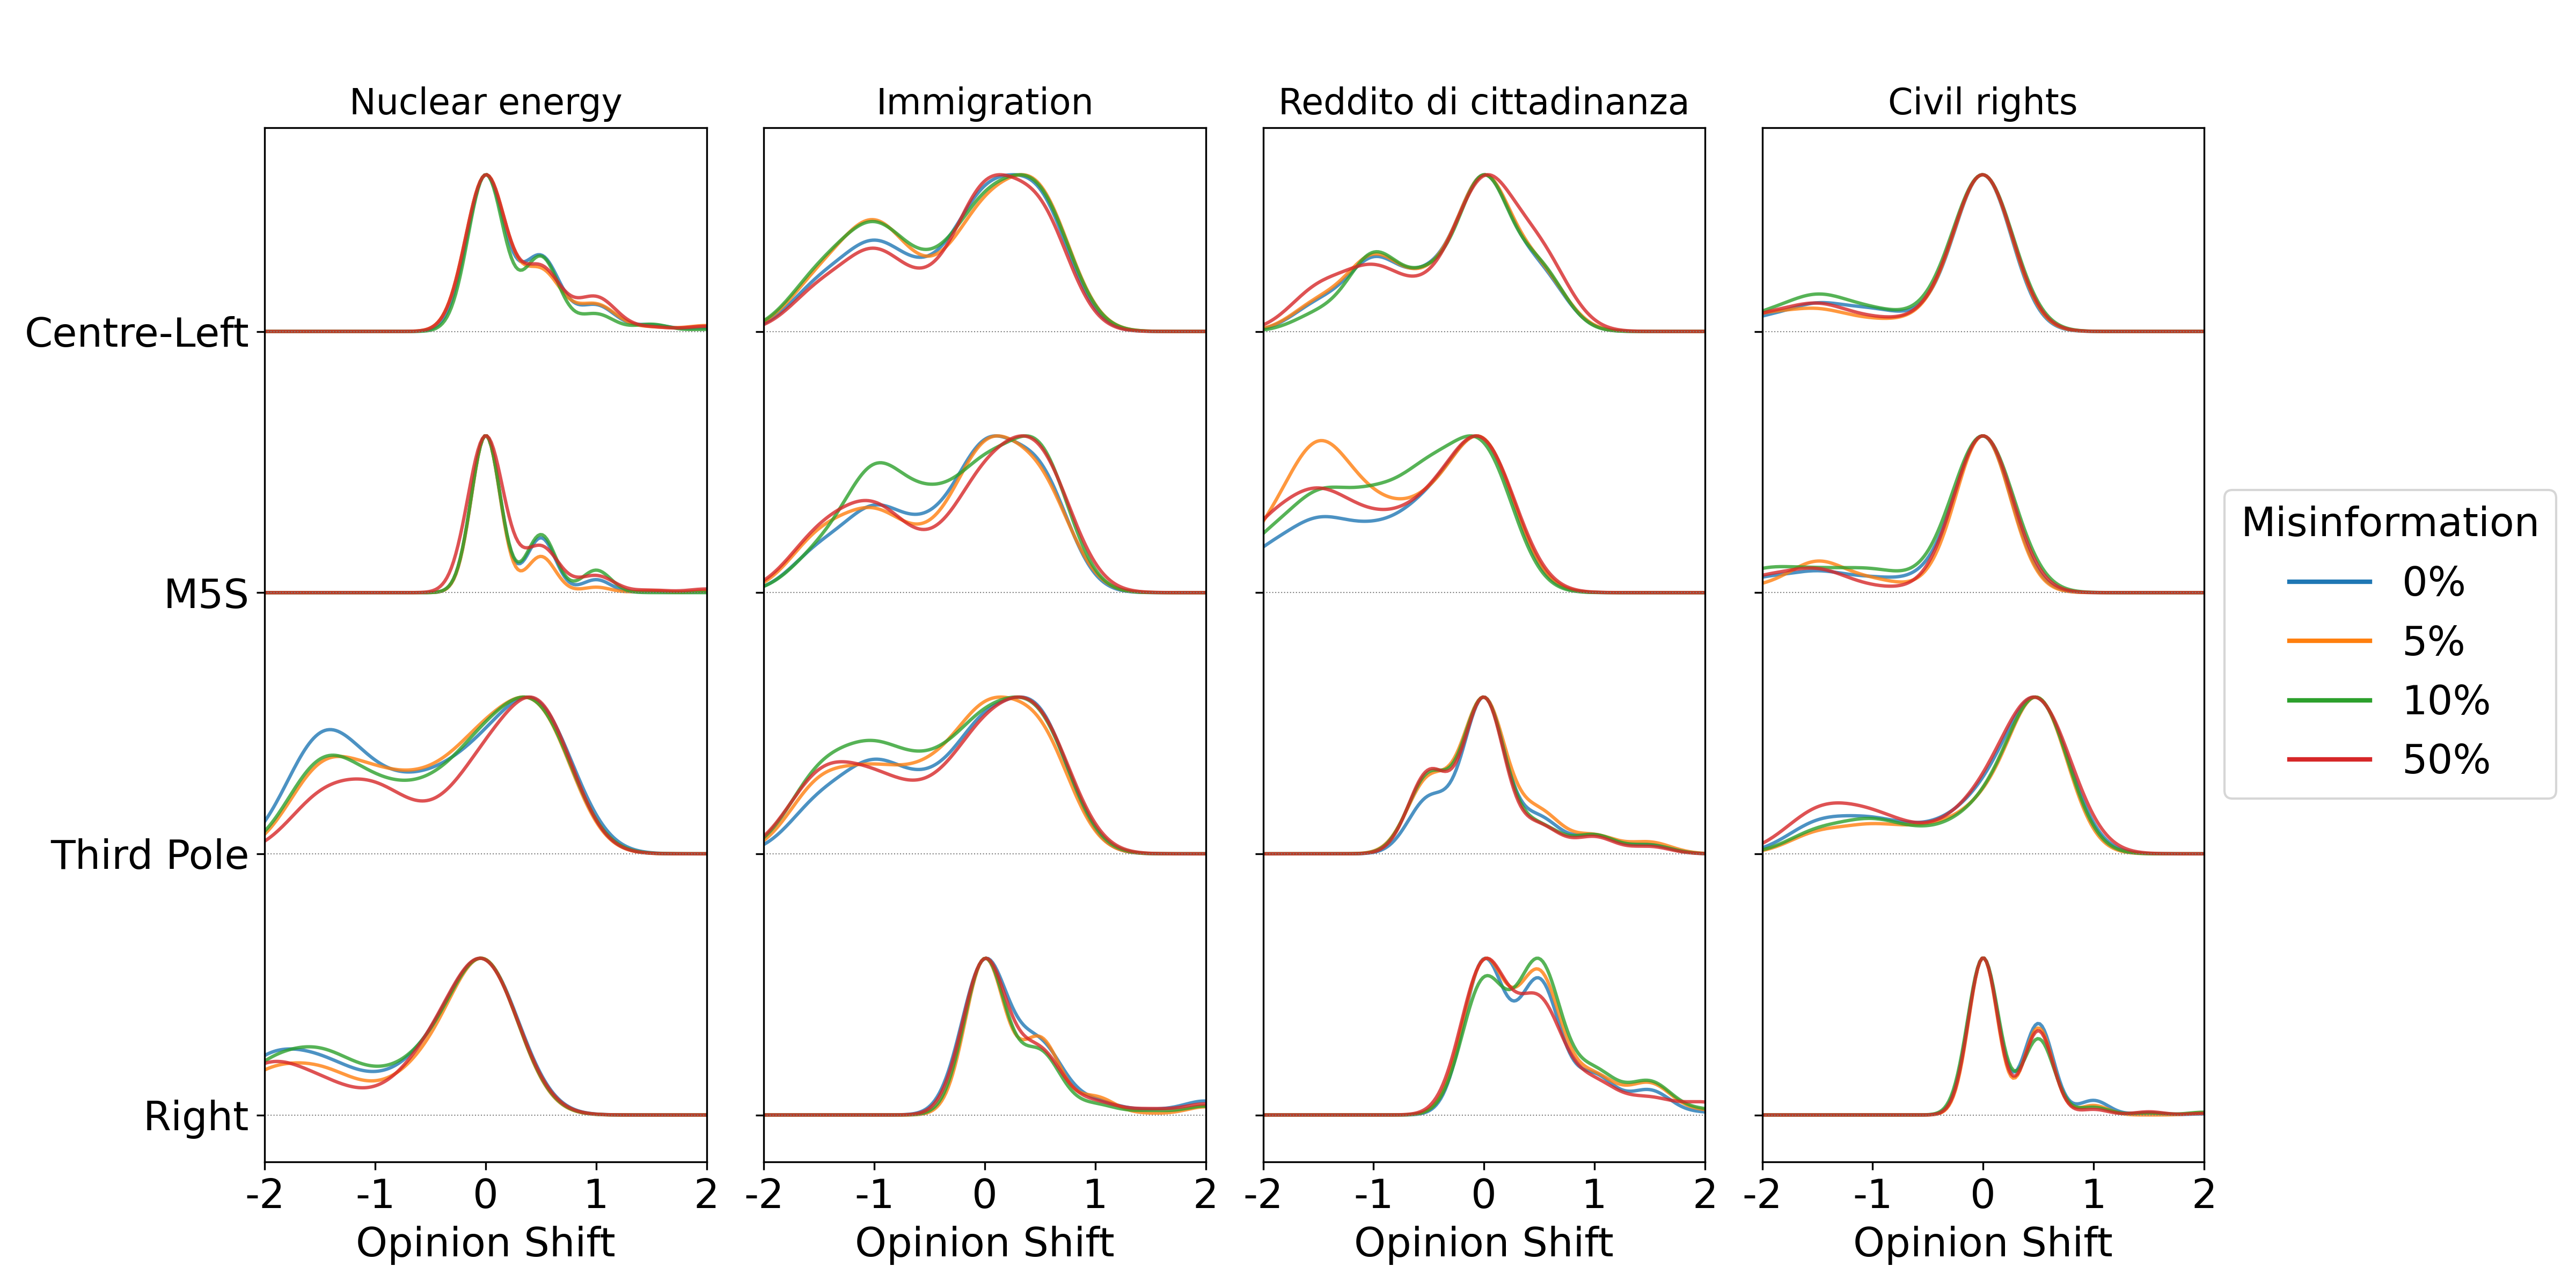
\includegraphics[width=0.8\linewidth]{Images/Misinformation/score_llm_RandomRecSys.png}
    \caption{
    Distribution of opinion shift (difference between final and initial opinion) for each topic an coalition, with varying levels of misinformation.
    The curves, which are almost completely overlapping, show that the presence of misinformation (up to 50\%) doesn't generate significant shifts in the opinions of LLM agents.
    Right coalition shows narrower distributions centered around zero, indicating greater resistance to change.
    }
    \label{fig:misinfo_opinion_shift}
\end{figure}


% Toxicity analysis
\subsection{Toxicity analysis}
To analyze the toxicity of generated content, the Detoxify library \cite{hanu2020detoxify} was used. This widely adopted tool detects offensive or harmful language in text and provides a continuous toxicity score between 0 and 1.
This section explores two aspects of the toxicity in the simulations: how it varies depending on whether users interact with in-group or out-group users, and how it differs across political coalitions and content types.

\subsection{Toxicity Toward In-Group vs Out-Group}
To analyze the toxicity of comments, for each user we computed the difference between the average toxicity of replies to users from the same coalition (in-group) and those directed at users from different coalitions (out-group).
The resulting distribution is visible in Figure \ref{fig:toxicity_in_out}.
To improve readability, toxicity values were normalized according to a logarithmic scale, since original values follow an exponential distribution: $log(toxicity + 1)$.

Looking at the plot, we can see that both distributions, one for the simulated content and one for the real data, are centered around zero.
This suggests that, on average, users don't show a strong difference in behavior when replying to in-group or out-group members.

However, the distribution of the simulated data is narrower and concentrated near zero.
This means that most agents behave in a similar way, with small variations in the toxicity difference between groups.

In contrast, the real data show a wider distribution: some users are more hostile way toward other coalitions, while others show more toxic behavior toward people supporting the same coalition.
This indicates a greater variety of behaviors in real-world interactions.

It's also possible to notice that both curves have a slight shift to the right, which may suggest a slight tendency to be more toxic toward out-group members. However, this effect is minimal.

Overall, the simulations fail to reproduce the diversity of behaviors observed in real data. 
In the scenarios studies, LLMs tend to behave in a uniform way and are not able to capture the differences in hostility toward different groups.


\begin{figure}[h]
    \centering
    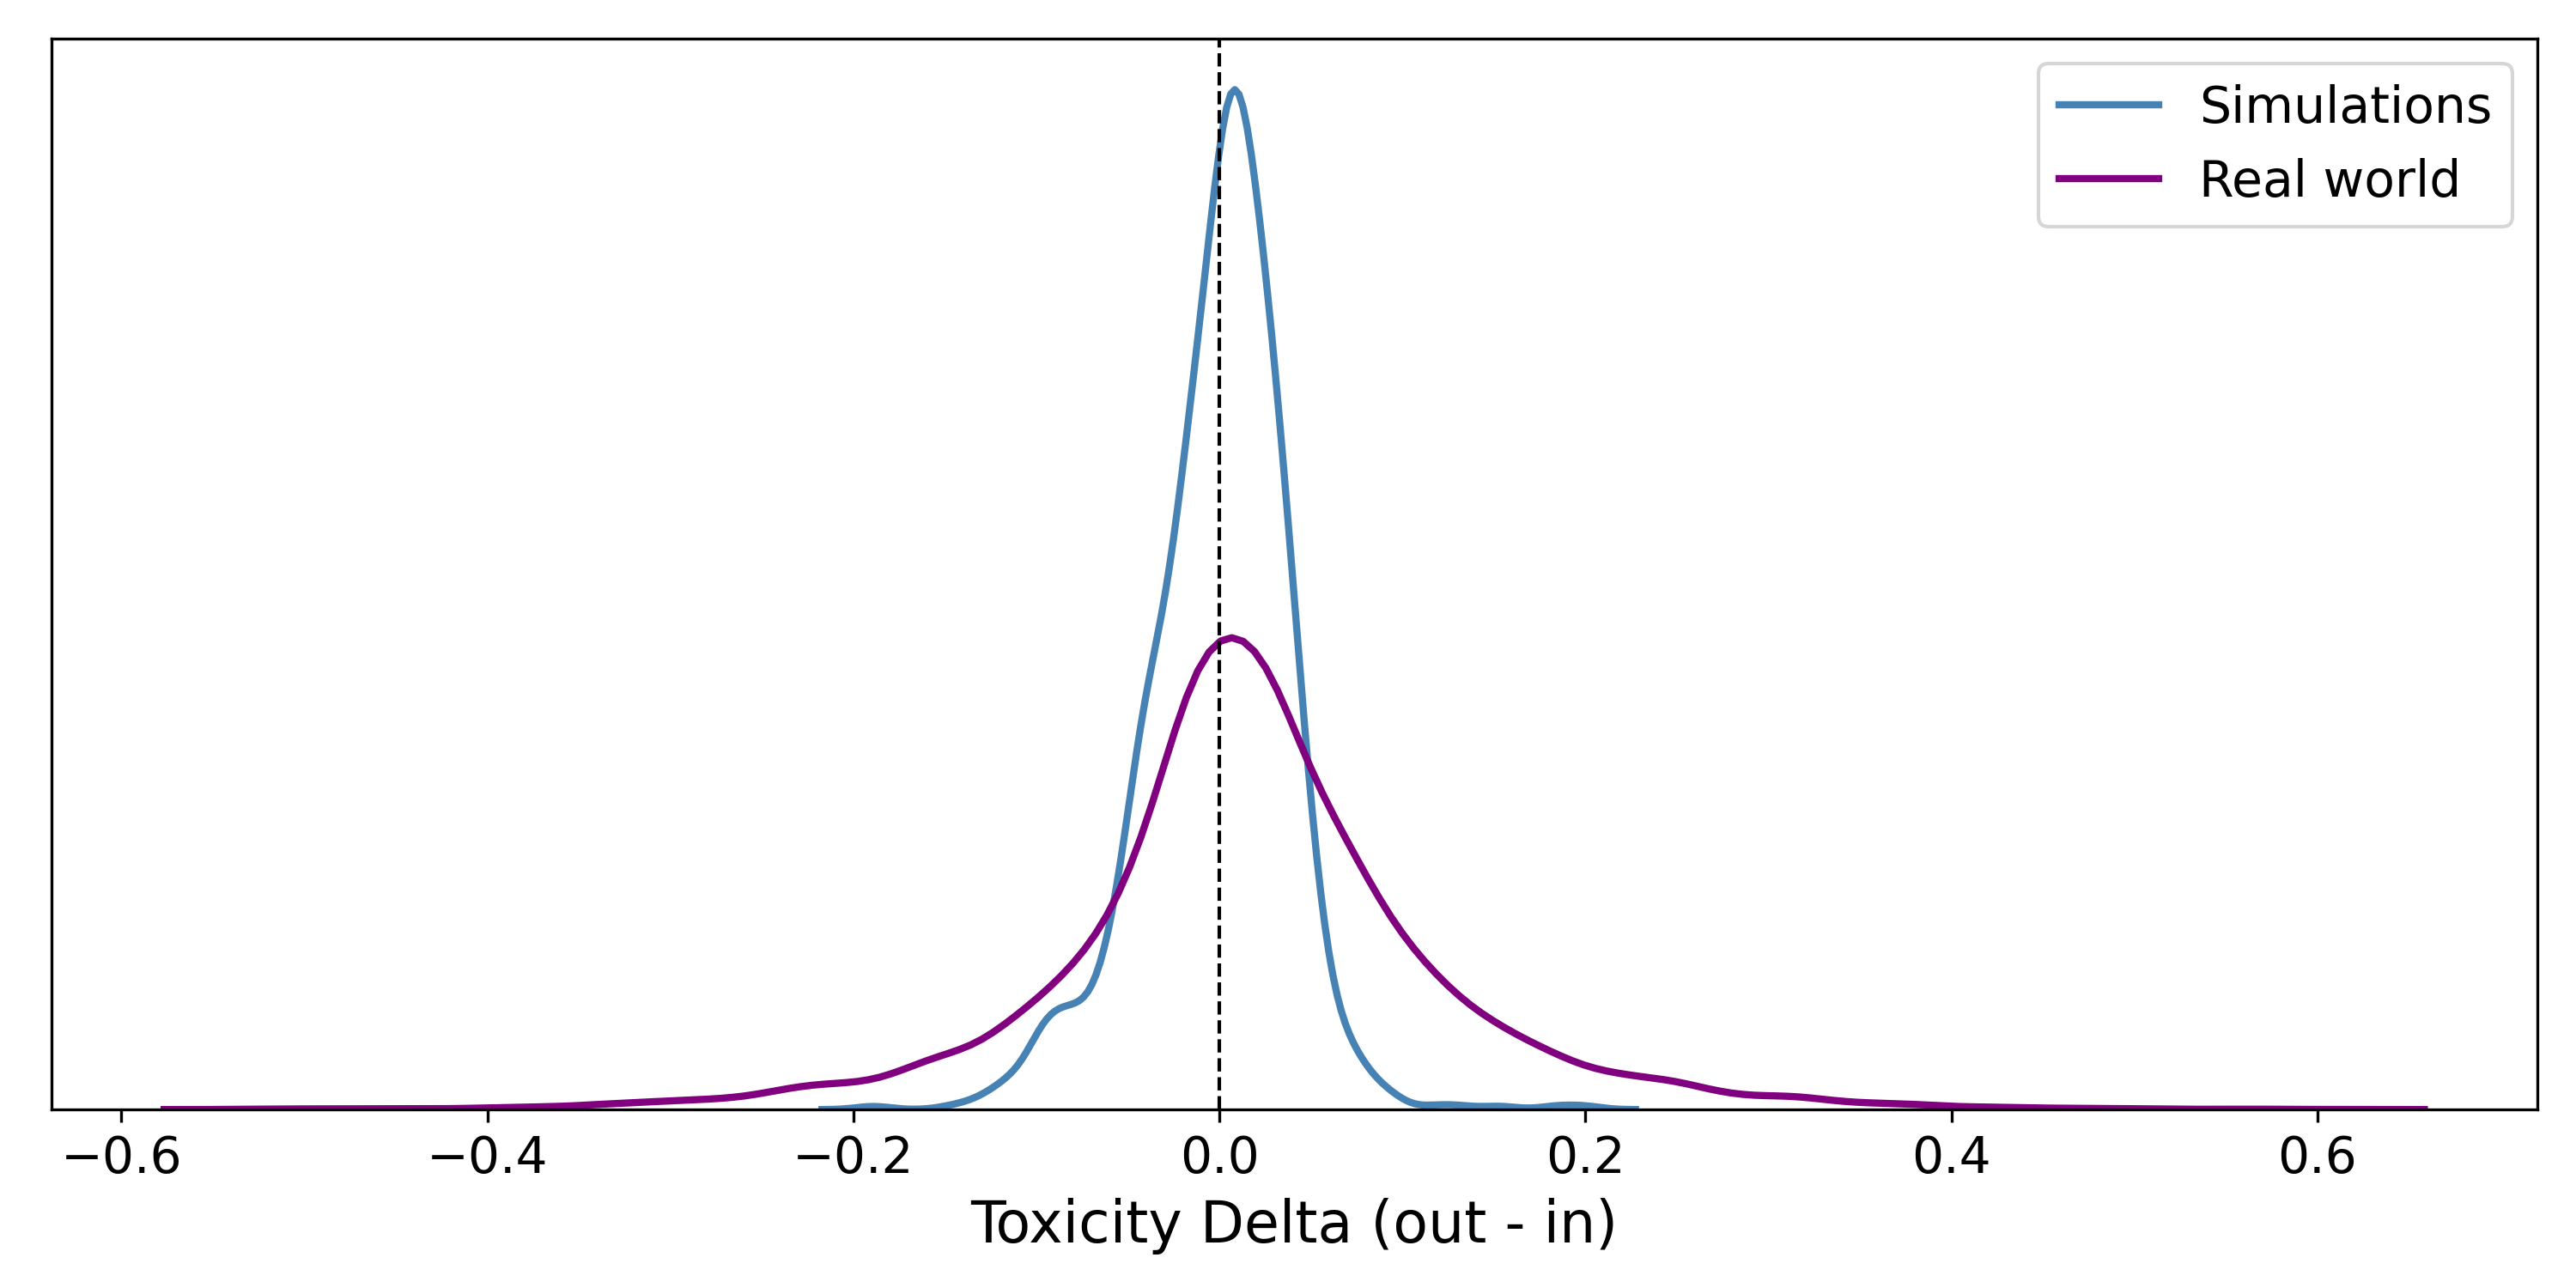
\includegraphics[width=0.6\linewidth]{Images/Toxicity/diff_in_out_combined.png}
    \caption{
    Distribution of the difference in mean toxicity toward out-group and in-group in user comments.
    The distribution of simulated content is more centered and narrow, indicating that agents behave similarly across groups.
    Real-wold data show greater variance, suggesting that some users are more hostile toward one of the two groups.
    }
    \label{fig:toxicity_in_out}
\end{figure}


\subsection{Toxicity Across Coalitions and Content Types}
The analysis of toxicity in texts generated by LLMs, divided by post and comments and categorized by political coalition, is visible in Figure \ref{fig:toxicity_box}, and reveals some interesting dynamics in the communication style of the agents within the simulations.

In general, posts tend to be more toxic on average than comments, with an a single exception: the Right coalition.
In this case, the generated comments are more toxic than the posts, suggesting that the the Right tends to bring more conflictual contributions to the conversations.
The Right coalition also shows the greatest variance in comment toxicity.
This suggests that their replies are more heterogeneous and can include extremely toxic texts.

The M5S coalition exhibits the greatest average toxicity in posts.
In addition, the distribution shows a visible positive skew, indicating that, beyond the generally more aggressive tone, there are also occasional posts with high levels of toxicity.

In contrast, the Centre-Left and Third Pole coalitions maintain a more moderate and stable tone, across both comments and posts.

Another important insight from this analysis concerns the shape of the toxicity distribution.
In all cases, the data shows a relevant positive skew: most texts have very low toxicity, but there are long tails extending toward higher values.
This pattern becomes particularly evident when using a logarithmic scale on the y axis, which makes these cases more visible.
This suggests that, despite the generally low average toxicity, LLMs can still produce highly toxic content, even though at lower frequency.

This ability to generate even highly toxic texts, maybe facilitated by the use of an uncensored language model, is beneficial in the context of social media simulations, as it allows a more realistic modeling of online conversations.


\begin{figure}[h]
    \centering
    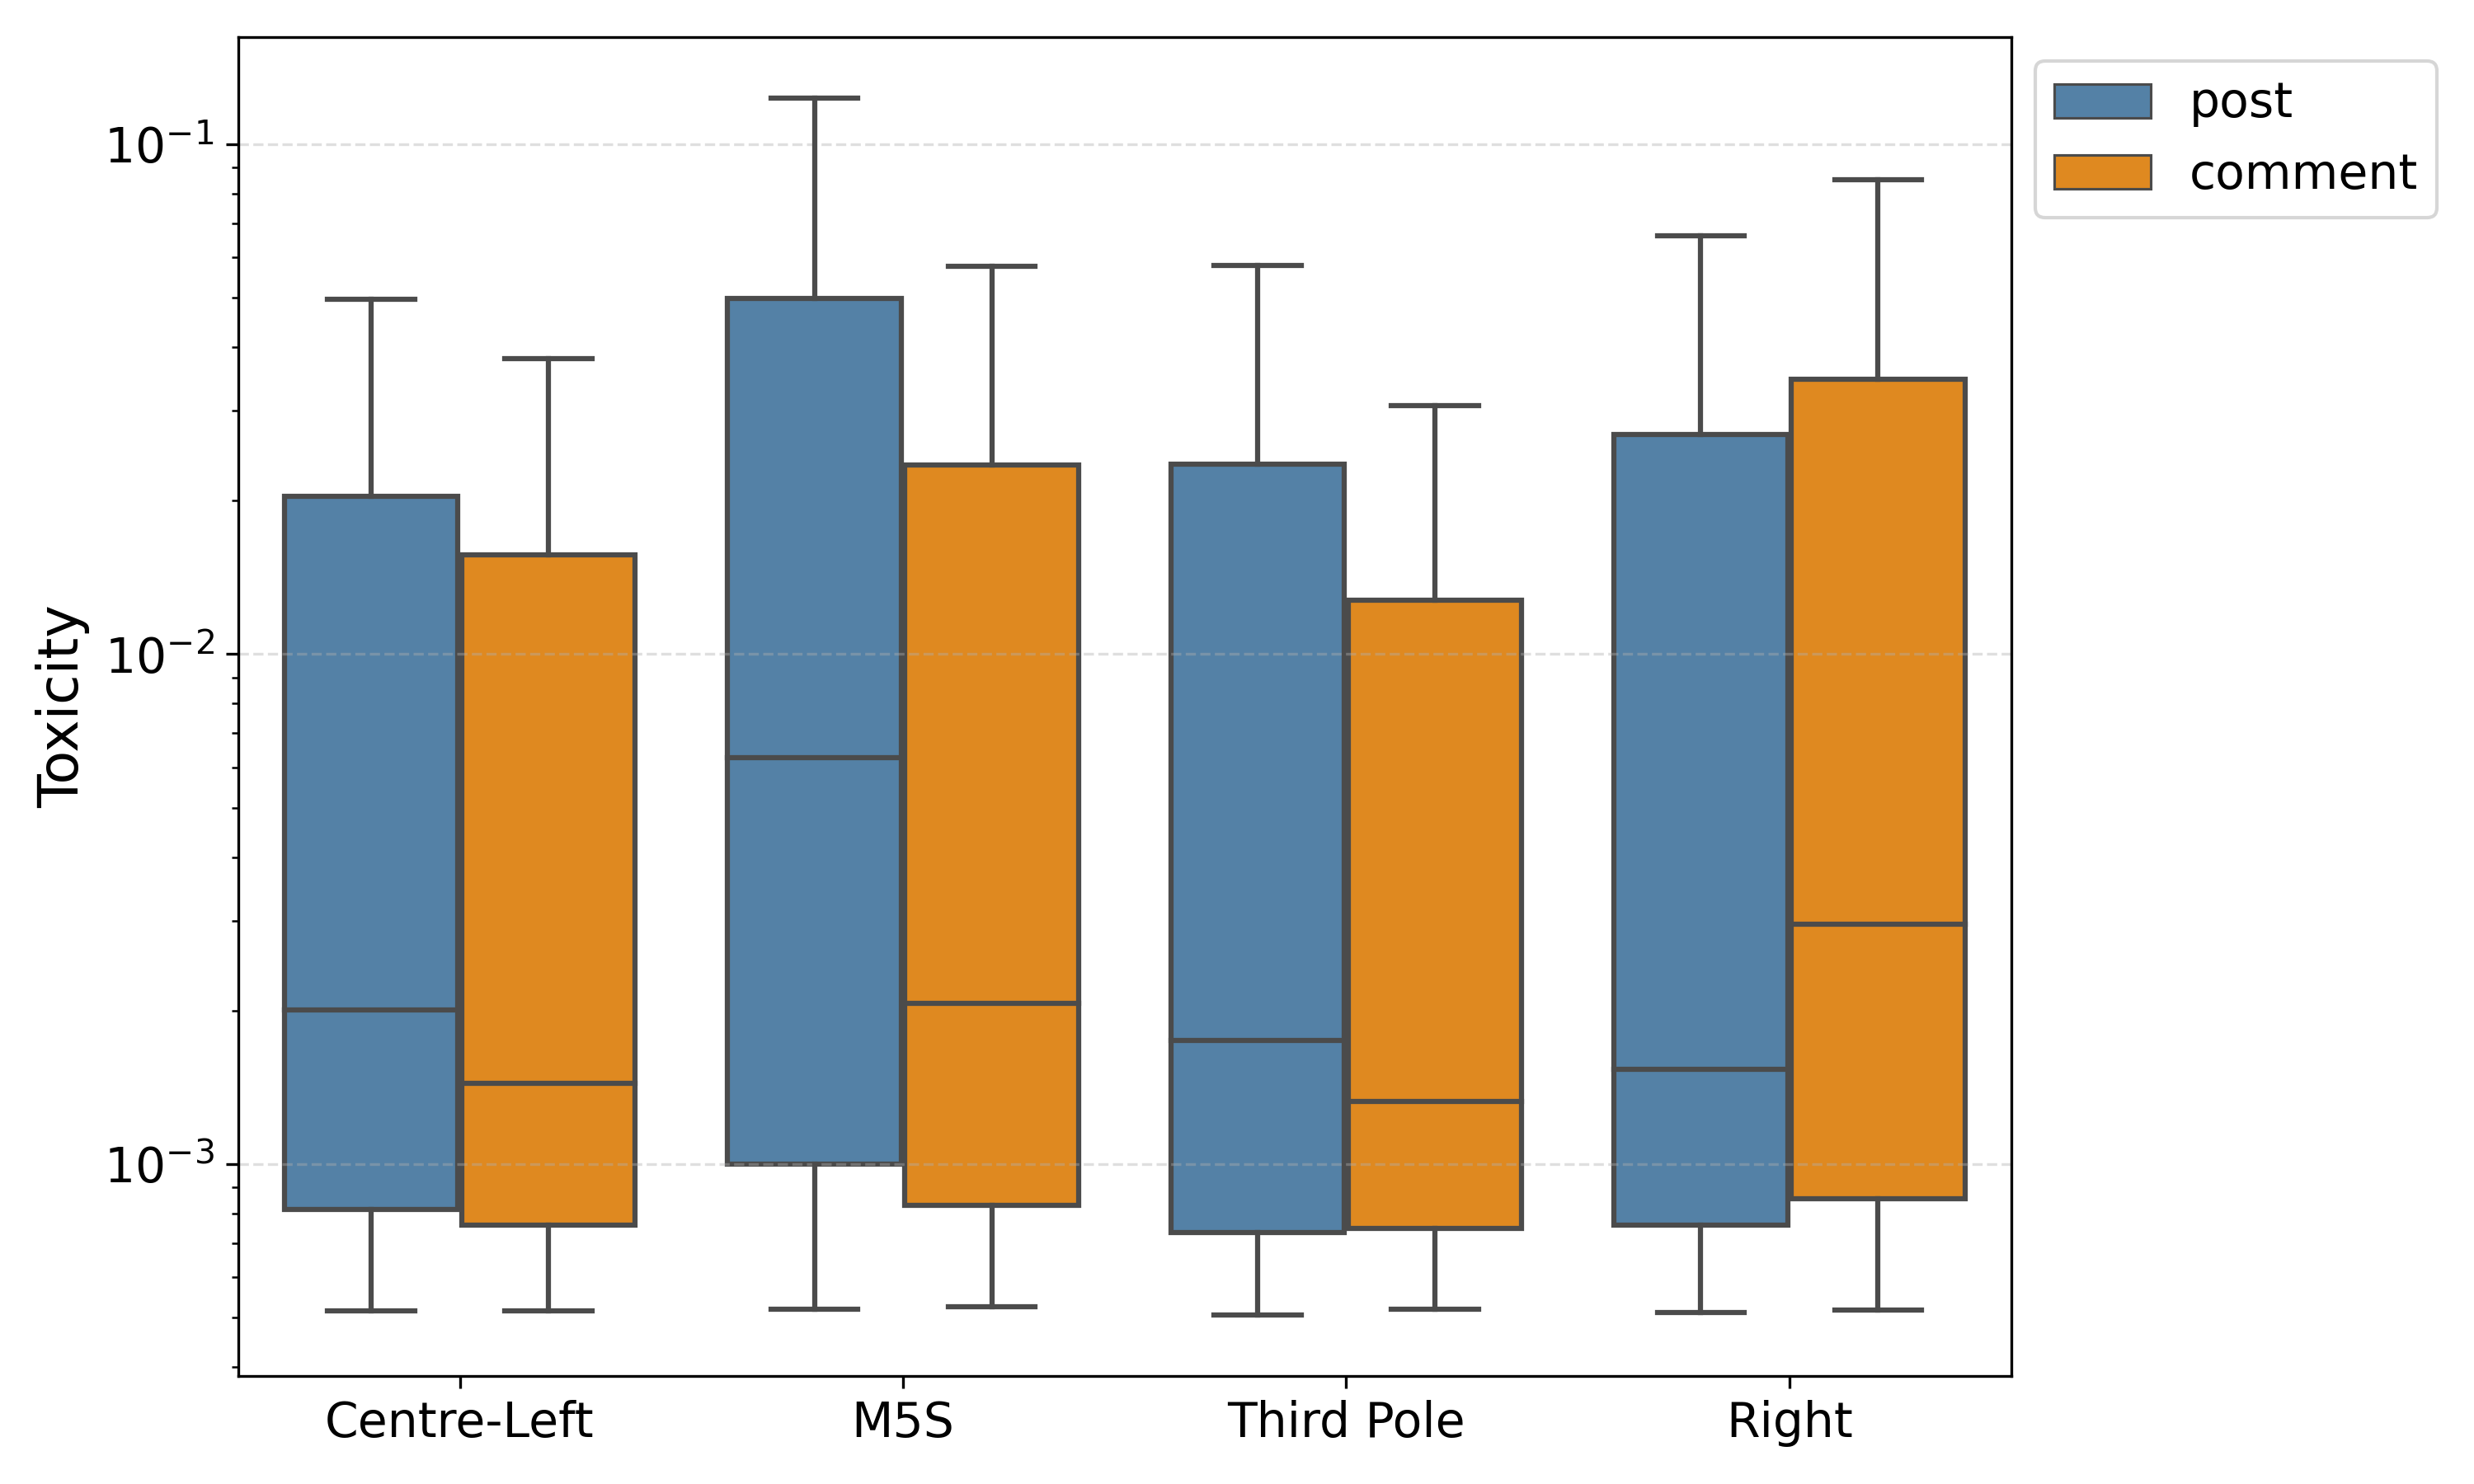
\includegraphics[width=0.6\linewidth]{Images/Toxicity/box_posts_vs_comments.png}
    \caption{
    Toxicity of LLM-generated texts, in posts and comments per political coalition.
    The y axis is in logarithmic scale to highlight the skew of the distribution.
    The Centre-Left and Third Pole coalitions have more stable and moderate tones.
    M5S is the most toxic in posts, while the Right generates comments with greater variability and toxicity.
    The long tails in all cases indicate that LLMs can generate content extremely toxic, even if rarely.
    }
    \label{fig:toxicity_box}
\end{figure}


% Recsys
\subsection{Content Recommendation Algorithms}
A comparison of the two content recommendation algorithms on the previously presented plots doesn't highlight any significant difference.
This happens because, at the beginning of the simulation, agents are not connected, so the network is empty.
Therefore, the used recommended system, \textit{ReverseChronoFollowersPopularity}, which should promote popular content from followers, doesn't have enough information to provide the best content.
In this initial phase, its behavior is similar to \textit{ContentRecSys}, the algorithm that suggests random content.

As a result, the different effects of the recommendation systems cannot emerge in the first few virtual days, and the dynamics produced by the two approaches are the same.
To see a real impact of the different recommender systems, simulations should run on a longer virtual time, or a network should be initialized with preexisting connections, providing a complete context of the initial user preferences.

This would allow a better evaluation of the impact of content selection on social networks.